\subsection{Kernel source management tools}

\begin{frame}
  \frametitle{Cscope}
  \begin{itemize}
  \item Tool to browse source code (mainly C, but also C++ or Java)
  \item Supports huge projects like the Linux kernel. Typically takes less
    than 1 min. to index the whole Linux sources.
  \item In Linux kernel sources, two ways of running it:
    \begin{itemize}
    \item \code{cscope -Rk}\\
      All files for all architectures at once
    \item \code{make cscope}\\
      \code{cscope -d cscope.out}\\
      Only files for your current architecture
    \end{itemize}
  \item Allows searching for a symbol, a definition, functions,
    strings, files, etc.
  \item Integration with editors like \code{vim} and \code{emacs}.
  \item Dedicated graphical front-end: \code{KScope}
  \item \url{http://cscope.sourceforge.net/}
  \end{itemize}
\end{frame}

\begin{frame}
  \frametitle{Cscope screenshot}
  \begin{center}
    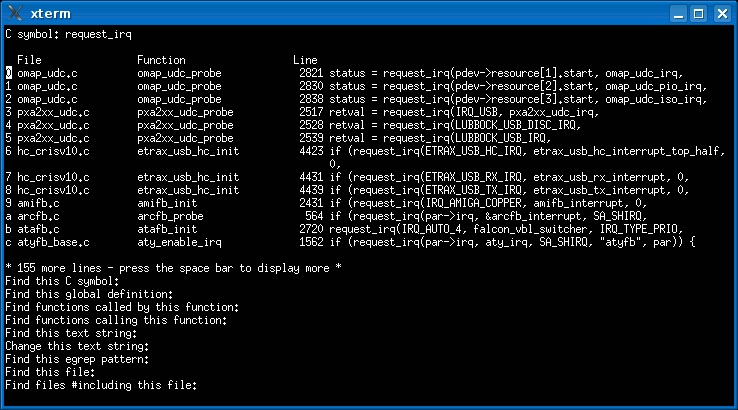
\includegraphics[width=\textwidth]{slides/kernel-source-code-management/cscope.png}
  \end{center}
  \code{[Tab]}: move the cursor between search results and commands\\
  \code{[Ctrl] [D]}: exit \code{cscope}
\end{frame}

\begin{frame}
  \frametitle{LXR: Linux Cross Reference}
  \begin{itemize}
  \item Generic source indexing tool and code browser
  \item Web server based, very easy and fast to use
  \item Very easy to find the declaration, implementation or usage
    of symbols
  \item Supports C and C++
  \item Supports huge code projects such as the Linux kernel (431 MB
    of source code in version 3.0).
  \item Takes a little time and patience to setup (configuration,
    indexing, web server configuration)
  \item You don't need to set up LXR by yourself. Use our
    \url{http://lxr.free-electrons.com} server!
  \item \url{http://sourceforge.net/projects/lxr}
  \end{itemize}
\end{frame}

\begin{frame}
  \frametitle{LXR screenshot}
  \begin{center}
    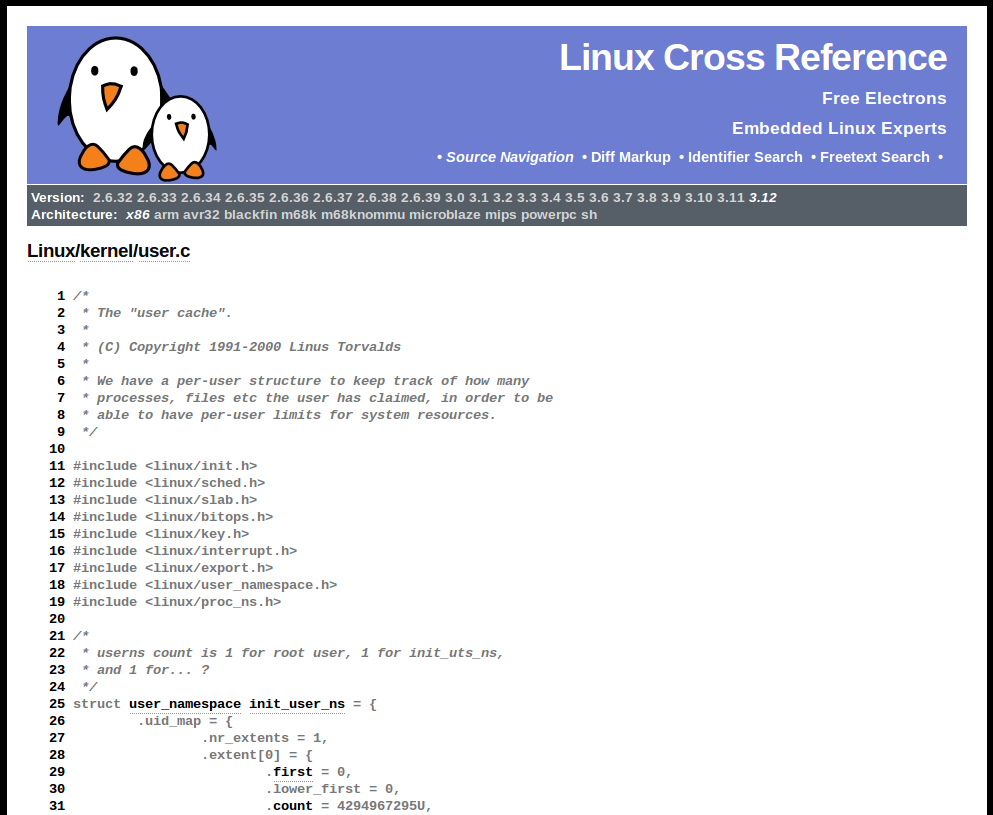
\includegraphics[height=0.8\textheight]{slides/kernel-source-code-management/lxr.png}
  \end{center}
\end{frame}
